% "{'classe':('PSI'),'chapitre':'dyn_inertie','type':('application'),'titre':'Triaxe', 'source':'','comp':['B2-10',],'corrige':True}"
%\setchapterimage{bandeau}
\chapter*{Application \arabic{cptApplication} \\ 
Triaxe -- \ifprof Corrigé \else Sujet \fi}
\addcontentsline{toc}{section}{Application \arabic{cptApplication} : Triaxe -- \ifprof Corrigé \else Sujet \fi}

\iflivret \stepcounter{cptApplication} \else
\ifprof  \stepcounter{cptApplication} \else \fi
\fi

\setcounter{question}{0}
%\marginnote{}
\marginnote[1cm]{
\UPSTIcompetence[2]{B2-10}
}
\begin{marginfigure}[3cm]
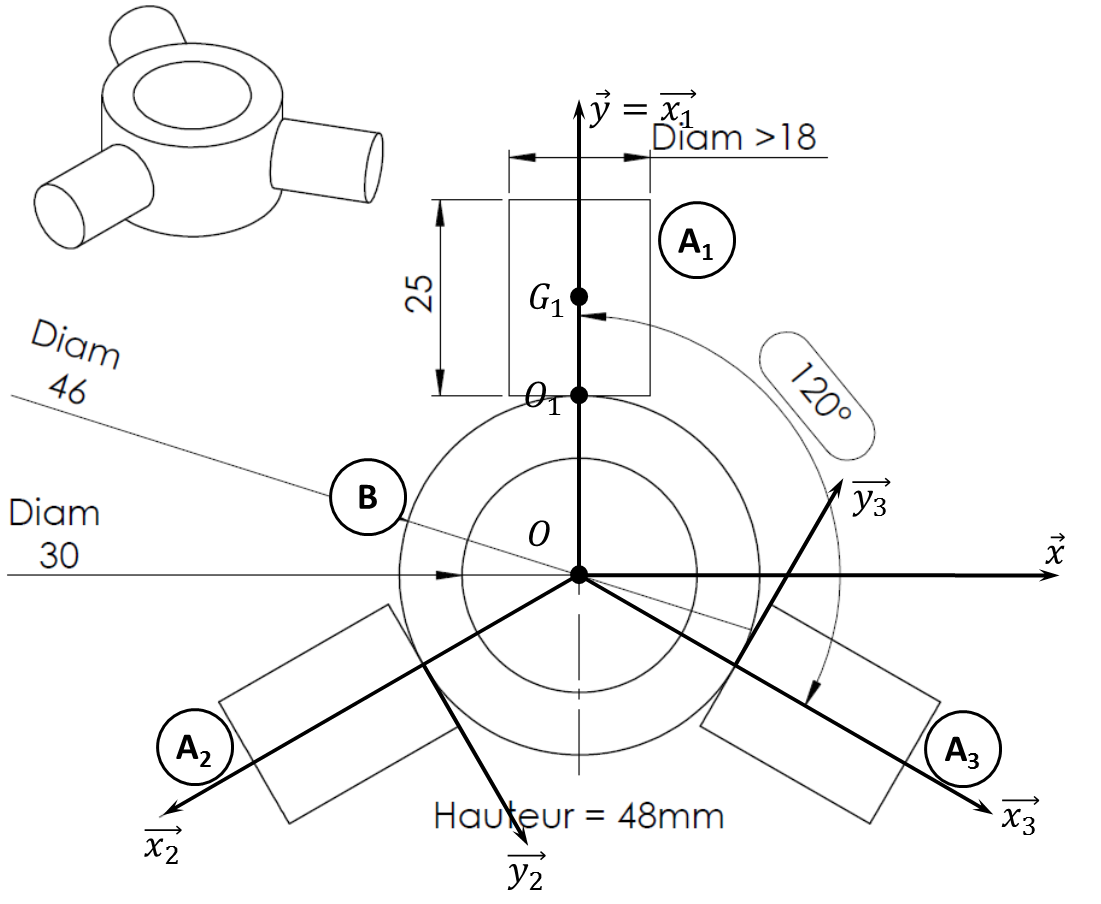
\includegraphics[width=4cm]{triaxe.png}
\end{marginfigure}



On donne le plan d'un triaxe constitué des 3 axes $A_1$, $A_2$, $A_3$ et du moyeu central noté $M$. On note  $T$ l'ensemble.

\begin{center}
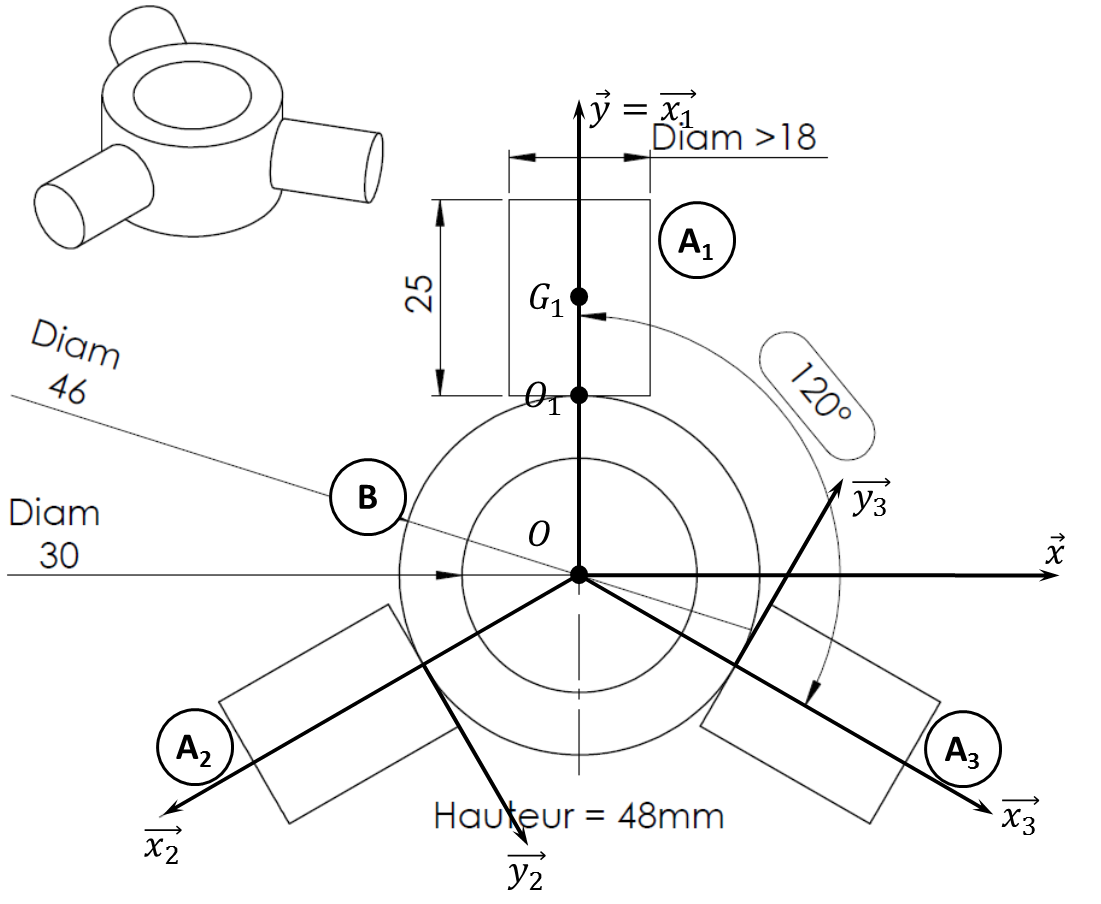
\includegraphics[width=8cm]{triaxe.png}
\end{center}
On note :
\begin{itemize}
\item $\vect{z}$ l'axe perpendiculaire au plan de la feuille. On se place ci-dessus dans le plan de symétrie $\left(O,\vect{x},\vect{y}\right)$;
\item $\rep{i}$ le repère $\repere{O_i}{x_i}{y_i}{z_i}$ et $\mathcal{B}_i$ la base associée.
\end{itemize}





\textbf{TOUS LES CALCULS SE FERONT DE MANIÈRE LITTERALE !}
\begin{itemize}
\item $D_1=\SI{18}{mm}$ et $H_1=\SI{25}{mm}$.
\item $D=\SI{46}{mm}$, $d=\SI{30}{mm}$ et $H=\SI{48}{mm}$.
\item $\alpha_1=\angl{x}{x_1}=90\degres$, $\alpha_2=\angl{x}{x_2}=-150\degres$ et 
$\alpha_3=\angl{x}{x_3}=-30\degres$.
\end{itemize}

On donne ci-dessous le paramétrage d'un axe $A_i$.

\begin{center}
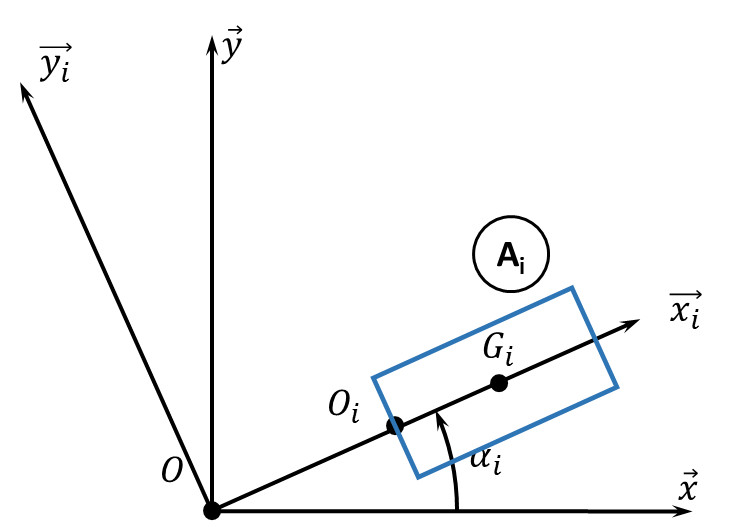
\includegraphics[width=7cm]{param.png}
\end{center}
\question{Déterminer (sans calcul) la position du centre de gravité du triaxe. }
\ifprof
\begin{corrige} ~\\

Le plan $\left(O,\vect{x},\vect{y}\right)$ est plan de symétrie du triaxe; donc $\vect{OG}\cdot\vect{z} =0$

Le plan $\left(O,\vect{y},\vect{z}\right)$ est plan de symétrie du triaxe; donc $\vect{OG}\cdot\vect{x} =0$

Reste la coordonnée selon $\vect{y}$. 

Les plans $\left(O,\vect{z},\vect{x_2}\right)$ et $\left(O,\vect{z},\vect{x_3}\right)$ étant plans de symétrie, on a 
 $\vect{OG}\cdot\vect{y_2} =0$ et  $\vect{OG}\cdot\vect{y_3} =0$. 
 Or $\vect{OG}= y_g \vect{y} =  y_g \cos \alpha_2 \vect{y_2} - y_g \sin \alpha_2 \vect{x_2}$. Il en résulte que   $y_g \cos \alpha_2 = 0$ et donc nécessairement $y_g=0$ car $\alpha_2\neq 0$. 
\end{corrige}
\else
\fi



\question{Déterminer analytiquement la position du centre de gravité $G_i$ du solide $A_i$ dans le repère $\rep{i}$.}
\ifprof
\begin{corrige}
On pourrait répondre directement en disant que le solide à 3 plans de symétrie orthogonaux entre eux. 
En utilisant la définition on a :
\begin{itemize}
\item $M_1 =\mu H_1\pi \dfrac{D_1^2}{4}$;
\item en coordonnées cylindriques, $\vect{O_iP_i}=x\vect{x_i}+ \rho \cos\theta \vect{y_i}+\rho \sin\theta \vect{z_i}$ et $\dd V = \rho\dd \rho \dd \theta \dd x$ avec $x\in[0,H_1]$, $\theta\in [0,2\pi]$, $\rho \in \left[0,D_1/2\right]$;
\item $m_ix_{G_i}=\mu \iiint x_P dV = \mu \iiint x  \rho\dd \rho \dd \theta \dd x= \mu \dfrac{H_1^2}{2} 2\pi \dfrac{D_1^2}{8}$;
\item $m_iy_{G_i}=\mu \iiint y_P dV = \mu \iiint \rho \cos\theta   \rho\dd \rho \dd \theta \dd x=0$;
\item $m_iz_{G_i}=\mu \iiint z_P dV = \mu \iiint \rho \sin\theta  \rho\dd \rho \dd \theta \dd x=0$. 
\end{itemize}
Au final,  $\mu H_1\pi  \dfrac{D_1^2}{4}x_{G_1}=\mu \dfrac{H_1^2}{2}  2\pi  \dfrac{D_1^2}{8} \Leftrightarrow   x_{G_1}= \dfrac{H_1}{2}$.
\end{corrige}
\else
\fi


\question{Déterminer (sans calcul) la \textbf{forme} de la matrice d'inertie du triaxe.}
\ifprof
\begin{corrige}

Le plan $\left(O,\vect{x},\vect{y}\right)$ est plan de symétrie du triaxe; donc $E = \iiint xz \dd m = 0 $ et $D = \iiint yz \dd m = 0 $.

Le plan $\left(O,\vect{y},\vect{z}\right)$ est plan de symétrie du triaxe; donc $E = \iiint xz \dd m = 0 $ et $F = \iiint xy \dd m = 0 $.

La matrice est donc diagonale et de la forme $\matinertie{A}{B}{C}{0}{0}{0}{\rep{}}$.

\end{corrige}
\else
\fi

\question{Déterminer analytiquement la matrice d'inertie du solide $A_i$ en $G_
i$ dans $\rep{i}$. On la note $\inertie{G_i}{A_i}=\matinertie{A_i}{B_i}{C_i}{-D_i}{-E_i}{-F_i}{\rep{i}}$ où les constantes seront à déterminer littéralement.}
\ifprof
\begin{corrige}
Le solide étant axisymétrique, on a : $D_i=E_i=F_i = 0$ et $C_i=B_i$. D'où  $\inertie{G_i}{A_1}=\matinertie{A_i}{B_i}{B_i}{0}{0}{0}{\rep{1}}$.

Calculons $A_i = \iiint \left(y^2+z^2\right)  \dd m=\mu \iiint \left(\rho^2\cos^2\theta +\rho^2\sin^2\theta\right) \rho \dd \rho \dd \theta \dd x  $

$ = \mu \iiint \rho^3  \dd \rho \dd \theta \dd z  = \mu \left[ \dfrac{\rho^4}{4}\right]_{0}^{D_1/2}2\pi H_1 = \mu \dfrac{D_1^4}{16\cdot 4}2\pi H_1 = M_1 \dfrac{D_1^2}{8}$.


Calculons $B_i = \iiint \left(x^2+z^2\right)  \dd m=\mu \iiint \left(x^2 +\rho^2\sin^2\theta\right) \rho \dd \rho \dd \theta \dd x$ 

$B_x=\mu \iiint x^2  \rho \dd \rho \dd \theta \dd x+\mu \iiint \rho^2\sin^2\theta \rho \dd \rho \dd \theta \dd x  $
$=\mu \iiint x^2  \rho \dd \rho \dd \theta \dd x = \mu \dfrac{H_1^3}{4\cdot 3}\dfrac{D_1^2}{8} 2\pi  = M  \dfrac{H_1^2}{12}   $

$B_z =\mu \iiint \rho^2\sin^2\theta \rho \dd \rho \dd \theta \dd x =\mu \iiint \rho^3\dfrac{1-\cos 2x}{2}\theta  \dd \rho \dd \theta \dd x=\mu \iiint \dfrac{\rho^3}{2}\theta  \dd \rho \dd \theta \dd x =\mu \dfrac{D_i^4}{2\cdot 16\cdot 4}2 \pi H_1 =M  \dfrac{D_i^2}{16}$.

Au final, $A_i =M_1 \dfrac{D_1^2}{8}$ et  $B_i =M\left(\dfrac{H_1^2}{12} + \dfrac{D_1^2}{16} \right)$.

%$\mu  \iiint y^2 \dd V +\mu  \iiint z^2 \dd V $.

%$ \mu  \iiint y^2 \dd V =  \mu  \iiint  \rho^2\cos^2\theta \dd V $ 
%$ = \mu  \iiint  \rho^2 \dd V \;  \iiint  \cos^2\theta \dd V  $

%$ = \mu  \iiint  \rho^3   \dfrac{1+\cos2\theta }{2} \dd \rho \dd \theta \dd z   $
%$ = \dfrac{\mu}{2}  \iiint     \rho^3+\rho^3\cos2\theta \dd \rho \dd \theta \dd z   $

%$ = \dfrac{\mu}{2} \left(\dfrac{D_1^4}{16\cdot 4} 2\pi H_1  +  \dfrac{D_1^4}{16\cdot 4} \left[ \dfrac{\sin 2 \theta}{2}\right]_{0}^{2\pi} H_1\right) = \dfrac{\mu}{2} \dfrac{D_1^4}{16\cdot 4} 2\pi H_1  =M_1 \dfrac{D_1^2}{16}  $

\end{corrige}
\else
\fi

\question{Déterminer $\inertie{G_i}{A_i}$ dans la base $\mathcal{B}\base{x}{y}{z}$ puis 
$\inertie{O}{A_i}$ dans la base $\mathcal{B}$.}
\ifprof
\begin{corrige}
 On a $\vect{x_i}=\cos\alpha\vect{x}+\sin\alpha\vect{y}$, $\vect{y_i}=\cos\alpha\vect{y}-\sin\alpha\vect{x}$. 
 En conséquences, on a : 
$P_{10}=\begin{pmatrix} \cos \alpha & - \sin\alpha & 0 \\ \sin \alpha & \cos \alpha & 0 \\ 0 & 0 & 1 \\ \end{pmatrix}$. 
On a donc 
$\inertie{G_1}{A_1}_{\rep{}}=P_{10}^{-1}\inertie{G_1}{A_1}_{\rep{1}}P_{10}$. 

$\inertie{G_1}{A_1}_{\rep{}}=
\begin{pmatrix} \cos \alpha & \sin\alpha & 0 \\-\sin \alpha & \cos \alpha & 0 \\ 0 & 0 & 1 \\ \end{pmatrix}
\matinertie{A_1}{B_1}{B_1}{0}{0}{0}{\rep{1}}
\begin{pmatrix} \cos \alpha & - \sin\alpha & 0 \\ \sin \alpha & \cos \alpha & 0 \\ 0 & 0 & 1 \\ \end{pmatrix}
$

$=
\begin{pmatrix} \cos \alpha & \sin\alpha & 0 \\-\sin \alpha & \cos \alpha & 0 \\ 0 & 0 & 1 \\ \end{pmatrix}
\begin{pmatrix}A_1 \cos \alpha & -A_1 \sin\alpha & 0 \\ B_1\sin \alpha & B_1\cos \alpha & 0 \\ 0 & 0 & B_1 \\ \end{pmatrix}
$

$=
\begin{pmatrix}
A_1 \cos^2\alpha +B_1 \sin^2\alpha& -A_1 \sin\alpha\cos\alpha+B_1\cos\alpha\sin\alpha & 0 \\ 
-A_1\sin \alpha\cos\alpha+B_1\cos\alpha\sin\alpha  &A_1\sin^2\alpha+ B_1\cos^2 \alpha & 0 \\ 0 & 0 & B_1 \\ \end{pmatrix}
$

%\textbf{Attention, pour aller de $\vect{x_1}$ vers $\vect{x}$, $\alpha=-\alpha_1$.}
%Avec $\alpha=\pi/2$, 
%on a : $\inertie{G_1}{A_1}_{\rep{}}=\begin{pmatrix}
%B_1 &0 & 0 \\ 
%0 & A_1 & 0 \\
% 0 & 0 & B_1 \\\end{pmatrix}_{\rep{}}
%$.


Par ailleurs, $\vect{OG_i}=\dfrac{H+D}{2}\vect{x_i}=\dfrac{H+D}{2}\left(\cos\alpha \vect{x}+\sin\alpha \vect{y} \right)$; donc :

  $\inertie{O}{A_i}_{\rep{}}=\inertie{G_i}{A_i}_{\rep{}}+M_1\begin{pmatrix}
\left( \dfrac{H+D}{2} \sin \alpha \right)^2 &\left( \dfrac{H+D}{2} \cos \alpha \right) \left( \dfrac{H+D}{2} \sin \alpha \right) & 0 \\ 
\left( \dfrac{H+D}{2} \cos \alpha \right) \left( \dfrac{H+D}{2} \sin \alpha \right) & \left( \dfrac{H+D}{2} \cos \alpha \right)^2& 0 \\
 0 & 0 &\left( \dfrac{H+D}{2} \cos \alpha \right)^2+\left( \dfrac{H+D}{2} \sin \alpha \right)^2 \\\end{pmatrix}_{\rep{}}$.
 
 
  $\inertie{O}{A_i}_{\rep{}}=\inertie{G_i}{A_i}_{\rep{}}+M_1\begin{pmatrix}
\left( \dfrac{H+D}{2} \sin \alpha \right)^2 &\left( \dfrac{H+D}{2} \right) ^2 \cos \alpha \sin \alpha  & 0 \\ 
\left( \dfrac{H+D}{2} \right) ^2 \cos \alpha \sin \alpha  & \left( \dfrac{H+D}{2} \cos \alpha \right)^2& 0 \\
 0 & 0 &\left( \dfrac{H+D}{2}\right)^2 \\\end{pmatrix}_{\rep{}}$.
 

Au final, 
$
\inertie{O}{A_i}_{\rep{}}=$

$
\begin{pmatrix}
A_1 \cos^2\alpha +B_1 \sin^2\alpha + M_1\left( \dfrac{H+D}{2} \sin \alpha \right)^2 
& \left( B_1-A_1\right) \sin\alpha\cos\alpha +M_1\left( \dfrac{H+D}{2} \right) ^2 \cos \alpha \sin \alpha 
& 0 \\ 
\left( B_1-A_1\right) \sin\alpha\cos\alpha +M_1 \left( \dfrac{H+D}{2} \right) ^2 \cos \alpha \sin \alpha 
&A_1\sin^2\alpha+ B_1\cos^2 \alpha +M_1\left( \dfrac{H+D}{2} \cos \alpha \right)^2
& 0 \\ 
0 & 0 & B_1+M_1\left( \dfrac{H+D}{2}\right)^2 \\ \end{pmatrix}
$.

On note 
$\inertie{O}{A_i}_{\rep{}}=\matinertie{f(\alpha)}{g(\alpha)}{h(\alpha)}{0}{0}{fg(\alpha)}{\rep{}}$.

%Au final, 
%$\inertie{O}{A_1}_{\rep{}}=\matinertie{B_1+M_1\left( \dfrac{H+D}{2}\right)^2}{A_1}{B_1+M_1\left( \dfrac{H+D}{2}\right)^2}{0}{0}{0}{\rep{}}$.
 

%Par ailleurs, $\vect{OG_1}=\dfrac{H+D}{2}\vect{y}$; donc :
%  $\inertie{O}{A_1}_{\rep{}}=\matinertie{B_1}{A_1}{B_1}{0}{0}{0}{\rep{}}+M_1\begin{pmatrix}
%\left( \dfrac{H+D}{2}\right)^2 &0 & 0 \\ 
%0 & 0& 0 \\
% 0 & 0 & \left( \dfrac{H+D}{2}\right)^2 \\\end{pmatrix}_{\rep{}}$.
% 
%Au final, 
%$\inertie{O}{A_1}_{\rep{}}=\matinertie{B_1+M_1\left( \dfrac{H+D}{2}\right)^2}{A_1}{B_1+M_1\left( \dfrac{H+D}{2}\right)^2}{0}{0}{0}{\rep{}}$.
% 
\end{corrige}
\else
\fi

\question{Déterminer $\inertie{O}{B}$  dans la base $\mathcal{B}$.}



\question{Proposer une méthode pour déterminer le tenseur d'inertie du triaxe en $O$ dans la base $\mathcal{B}$.}

\question{Déterminer le tenseur d'inertie du triaxe en $O$ dans la base $\mathcal{B}$.}


%\subparagraph{}
%\textit{Déterminer $\inertie{O}{A_2}$  et $\inertie{O}{A_3}$ dans la base $\mathcal{B}\base{x}{y}{z}$.}
\ifprof

\begin{corrige}  ~\\
%
%
% $\inertie{G_2}{A_2}_{\rep{}}=
%\begin{pmatrix}
%A_1 \cos^2\alpha +B_1 \sin^2\alpha& -A_1 \sin\alpha\cos\alpha+B_1\cos\alpha\sin\alpha & 0 \\ 
%-A_1\sin \alpha\cos\alpha+B_1\cos\alpha\sin\alpha  &A_1\sin^2\alpha+ B_1\cos^2 \alpha & 0 \\ 0 & 0 & B_1 \\ \end{pmatrix}.$
%
%
%
%Avec $\alpha=-\pi/6$, 
%on a : 
% $\inertie{G_2}{A_2}_{\rep{}}=
%\begin{pmatrix}
% \dfrac{3A_1 + B_1}{4} & \left(A_1-B_1\right) \dfrac{\sqrt{3}}{4} & 0 \\ 
% \left(A_1-B_1\right) \dfrac{\sqrt{3}}{4}  &\dfrac{A_1+3B_1}{4}  & 0 \\ 0 & 0 & B_1 \\ \end{pmatrix}.$
%
%
%Par ailleurs, $\vect{OG_2}=\dfrac{H+D}{2}\cos\alpha\vect{x}+\dfrac{H+D}{2}\sin\alpha\vect{y}$; 
%
%
%donc :
%  $\inertie{O}{A_1}_{\rep{}}=\matinertie{B_1}{A_1}{B_1}{0}{0}{0}{\rep{}}+M_1\begin{pmatrix}
%\left( \dfrac{H+D}{2}\right)^2\dfrac{1}{4}  & -\dfrac{(H+D)^2}{4}\dfrac{\sqrt{3}}{4}  & 0 \\ 
%-\dfrac{(H+D)^2}{4}\dfrac{\sqrt{3}}{4}& \left( \dfrac{H+D}{2}\right)^2\dfrac{3}{4}& 0 \\
% 0 & 0 & \left( \dfrac{H+D}{2}\right)^2 \\\end{pmatrix}_{\rep{}}$.
% 
%
%%
%%Par ailleurs, $\vect{OG_2}=\dfrac{H+D}{2}\cos\alpha\vect{x}+\dfrac{H+D}{2}\sin\alpha\vect{y}$; 
%%
%%
%%donc :
%%  $\inertie{O}{A_1}_{\rep{}}=\matinertie{B_1}{A_1}{B_1}{0}{0}{0}{\rep{}}+M_1\begin{pmatrix}
%%\left( \dfrac{H+D}{2}\right)^2 \sin^2\alpha  & -\dfrac{(H+D)^2}{4}\cos\alpha\sin\alpha  & 0 \\ 
%%-\dfrac{(H+D)^2}{4}\cos\alpha\sin\alpha & \left( \dfrac{H+D}{2}\right)^2 \cos^2\alpha& 0 \\
%% 0 & 0 & \left( \dfrac{H+D}{2}\right)^2 \\\end{pmatrix}_{\rep{}}$.
%% 
%%Au final, 
%%$\inertie{O}{A_1}_{\rep{}}=\matinertie{B_1+M_1\left( \dfrac{H+D}{2}\right)^2}{A_1}{B_1+M_1\left( \dfrac{H+D}{2}\right)^2}{0}{0}{0}{\rep{}}$.
 
\end{corrige}
\else
\fi

\question{Déterminer $\inertie{O}{M}$  la matrice d'inertie du moyeu $M$.}
\ifprof
\begin{corrige}
 
\end{corrige}
\else
\fi

\ifprof
\else
\begin{marginfigure}
\centering

\includegraphics[width=3cm]{Cy_04_01_Application_02_Triaxe_qr}
\end{marginfigure}
\fi


\question{Déterminer $\inertie{O}{T}$  la matrice d'inertie du triaxe $T$.}
\ifprof
\begin{corrige}
 
\end{corrige}
\else
\fi
%
%
%On donne $\mu=\SI{7,8}{kg.dm^{-3}}$.
%\subparagraph{}
%\textit{Déterminer ce moment d'inertie.}
%\ifprof
%\begin{corrige}
%\end{corrige}
%\else
%\fi
%
%\subparagraph{}
%\textit{Indiquer la méthode pour déterminer le tenseur d'inertie en $O$ dans la base $\base{x}{y}{z}$ ($O$ étant situé au centre de la pièce).}
%\ifprof
%\begin{corrige}
%\end{corrige}
%\else
%%\fi
%%
%On donne $\mu=\SI{7,8}{kg.dm^{-3}}$.
%\subparagraph{}
%\textit{Déterminer ce moment d'inertie.}
%\ifprof
%\begin{corrige}
%\end{corrige}
%\else
%\fi
%Pour cette pièce, SolidWorks nous donne les informations suivantes. 
%\begin{center}
%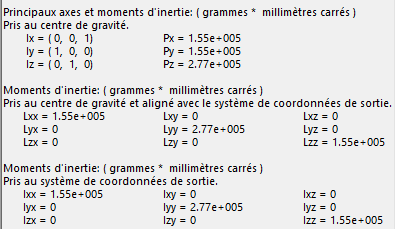
\includegraphics[width=.9\linewidth]{SW_04.png}
%\end{center}

%Propriétés de masse de TriAxe
%     Configuration: Défaut
%     Système de coordonnées: -- par défaut --
%
%Densité = 0.0078 grammes par millimètre cube
%
%Masse = 357 grammes
%
%Volume = 4.58e+004 millimètres cubes
%
%Superficie = 1.44e+004  millimètres carrés
%
%Centre de gravité: ( millimètres )
%	X = 0
%	Y = 0
%	Z = 0
%
%Principaux axes et moments d'inertie: ( grammes *  millimètres carrés )
%Pris au centre de gravité.
%	 Ix = ( 0,  0,  1)   	Px = 1.55e+005
%	 Iy = ( 1,  0,  0)   	Py = 1.55e+005
%	 Iz = ( 0,  1,  0)   	Pz = 2.77e+005
%
%Moments d'inertie: ( grammes *  millimètres carrés )
%Pris au centre de gravité et aligné avec le système de coordonnées de sortie.
%	Lxx = 1.55e+005	Lxy = 0	Lxz = 0
%	Lyx = 0	Lyy = 2.77e+005	Lyz = 0
%	Lzx = 0	Lzy = 0	Lzz = 1.55e+005
%
%Moments d'inertie: ( grammes *  millimètres carrés )
%Pris au système de coordonnées de sortie.
%	Ixx = 1.55e+005	Ixy = 0	Ixz = 0
%	Iyx = 0	Iyy = 2.77e+005	Iyz = 0
%	Izx = 0	Izy = 0	Izz = 1.55e+005
%\subparagraph{}
%\textit{Détailler ce que cela signifie.}
%\ifprof
%\begin{corrige}
%\end{corrige}
%\else
%
%
%


